\documentclass[12pt,a4paper]{article}
\usepackage{tikz}
\usepackage{times}
\usepackage[left=3cm, right=2cm, top=3cm, bottom=3cm]{geometry}
\usetikzlibrary{circuits.plc.sfc,calc,positioning}
\usetikzlibrary{circuits.plc.ladder} 
\usepackage[utf8]{vietnam}
 \tikzset{
    coil NA/.style={coil={#1,symbol={$/$}}},
    every coil/.style={minimum size=2.4\tikzcircuitssizeunit,coil ladder curvature=0.5},
    every coil S/.style={minimum size=2.4\tikzcircuitssizeunit,coil ladder curvature=0.5},
    every coil R/.style={minimum size=2.4\tikzcircuitssizeunit,coil ladder curvature=0.5},
    every coil NA/.style={minimum size=2.4\tikzcircuitssizeunit,coil ladder curvature=0.5}
}
\usepackage{circuitikz}
\usepackage{indentfirst}
\setlength{\parindent}{0cm}
\usepackage{caption}
\usepackage{hyperref}
\begin{document}

{
\textbf{\LARGE Bài tập cá nhân \#2}


\begin{tabbing}{}
    \setlength{\parindent}{1cm}
    Tên nhóm A \= Điều khiển góc phương vị của chảo vệ tinh \kill
    \textbf{Họ và tên} \> Nguyễn Đức Đạt\\
    \textbf{MSSV} \> 2111009
\end{tabbing}
}

MSSV định dạng XXYYZZZ là 2111009. Do đó XX = 21, YY = 11, ZZZ = 009.

\section{Mạch điều khiển}

\begin{figure}[ht]
\centering
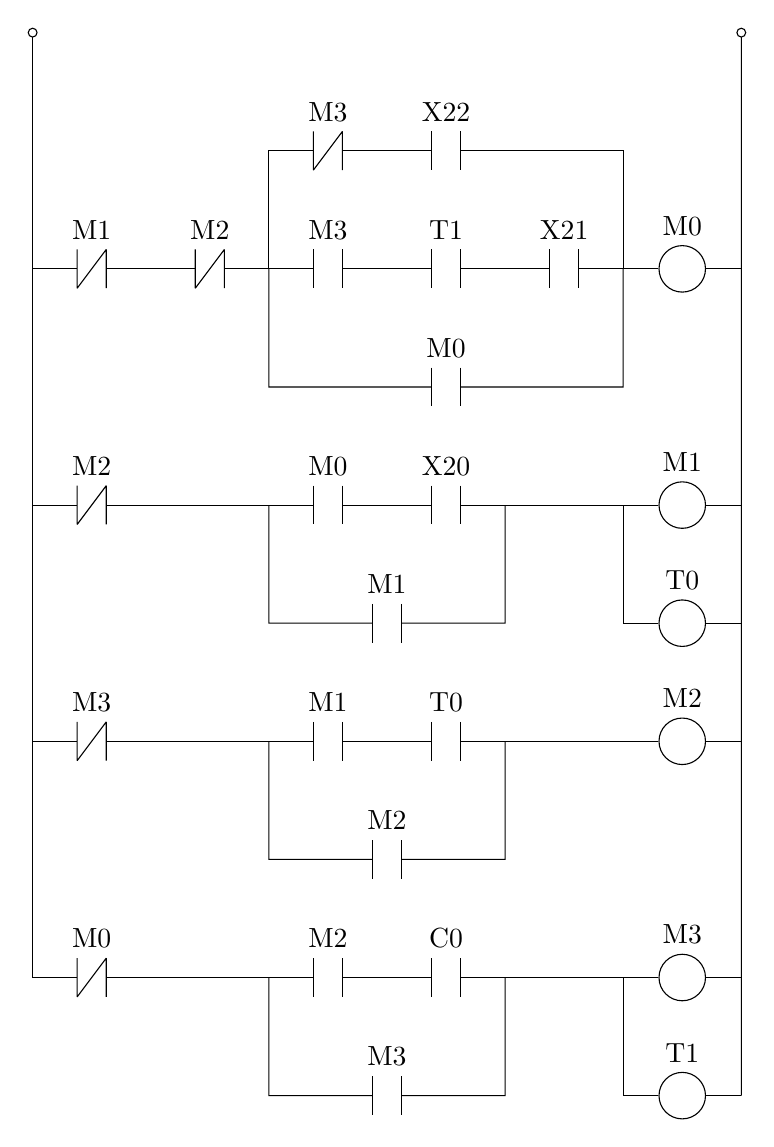
\begin{tikzpicture}[circuit plc ladder,x=1cm,y=1cm]
    \draw (0,0) to[contact NC={info=M1}] ++(1.5,0)
        to[contact NC={info=M2}] ++(1.5,0) coordinate (a)
        to[contact NO={info=M3}] ++(1.5,0)
        to[contact NO={info=T1}] ++(1.5,0)
        to[contact NO={info=X21}] ++ (1.5,0)
        to[coil={info=M0}] ++(1.5,0);
    \draw (a) -- ++(0,1.5) to[contact NC={info=M3}] ++ (1.5,0) to[contact NO={info=X22}] ++ (1.5,0) -- ++(1.5,0) -- ++(0,-1.5);
    \draw (a) -- ++(0,-1.5) to[contact NO={info=M0}] ++ (4.5,0) -- ++(0,1.5);

    \draw (0,-3) to[contact NC={info=M2}] ++(1.5,0) -- ++(1.5,0) coordinate (b)
        to[contact NO={info=M0}] ++(1.5,0)
        to[contact NO={info=X20}] ++(1.5,0) -- ++(1.5,0) coordinate (b')
        to[coil={info=M1}] ++(1.5,0);
    \draw (b) -- ++(0,-1.5) to[contact NO={info=M1}] ++ (3,0) -- ++(0,1.5);
    \draw (b') -- ++(0,-1.5) to[coil={info=T0}] ++ (1.5,0);


    \draw (0,-6) to[contact NC={info=M3}] ++(1.5,0) -- ++(1.5,0) coordinate (c)
        to[contact NO={info=M1}] ++(1.5,0)
        to[contact NO={info=T0}] ++(1.5,0) -- ++(1.5,0) coordinate (c')
        to[coil={info=M2}] ++(1.5,0);
    \draw (c) -- ++(0,-1.5) to[contact NO={info=M2}] ++ (3,0) -- ++(0,1.5);

    \draw (0,-9) to[contact NC={info=M0}] ++(1.5,0) -- ++(1.5,0) coordinate (d)
        to[contact NO={info=M2}] ++(1.5,0)
        to[contact NO={info=C0}] ++(1.5,0) -- ++(1.5,0) coordinate (d')
        to[coil={info=M3}] ++(1.5,0);
    \draw (d) -- ++(0,-1.5) to[contact NO={info=M3}] ++ (3,0) -- ++(0,1.5);
    \draw (d') -- ++(0,-1.5) to[coil={info=T1}] ++ (1.5,0);

    \draw (0,3) to[short,o-] ++(0,-12);
    \draw (9,3) to[short,o-] ++(0,-13.5);
\end{tikzpicture}
\end{figure}



Giải thích:
\begin{itemize}
    \item X22 là tiếp điểm thường mở của nút bấm PB3 đóng vai trò là nút khởi động.
    \item T0 có hằng số K210 do yêu cầu thời gian delay là XX = 21 giây.
    \item T1 có hằng số K9 do yêu cầu thời gian delay là ZZZ/10 = 0.9 giây.
\end{itemize}
\newpage
\section{Mạch động lực}

\begin{figure}[ht]
    \centering
    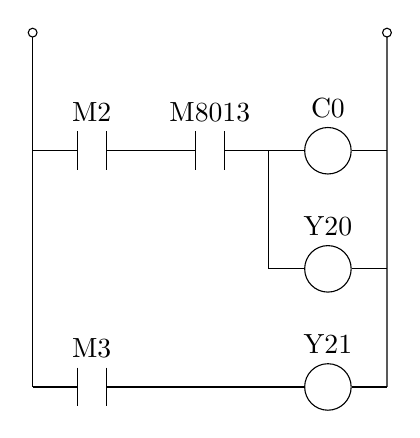
\begin{tikzpicture}[circuit plc ladder,x=1cm,y=1cm]
        \draw (0,0) to[contact NO={info=M2}] ++(1.5,0)
            to[contact NO={info=M8013}] ++(1.5,0)  coordinate(a)
            to[coil={info=C0}] ++(1.5,0);
        \draw (a) -- ++(0,-1.5) to[coil={info=Y20}] ++(1.5,0);

        \draw (0,-3) to[contact NO={info=M3}] ++(1.5,0) -- ++(1.5,0)
            to[coil={info=Y21}] ++(1.5,0);

        \draw (0,1.5) to[short,o-] ++(0,-4.5);
        \draw (4.5,1.5) to[short,o-] ++(0,-4.5);
    \end{tikzpicture}
\end{figure}

Giải thích:
\begin{itemize}
    \item C0 có hằng số là K11 do yêu cầu số lần chớp tắt là YY = 11 lần.
\end{itemize}

\section{Mô phỏng trên SW0D5C-FXTRN-BEG}
Video mô phỏng mạch bên dưới tại đường dẫn \url{https://youtu.be/m5hOxP-cvJk}.
\begin{center}
    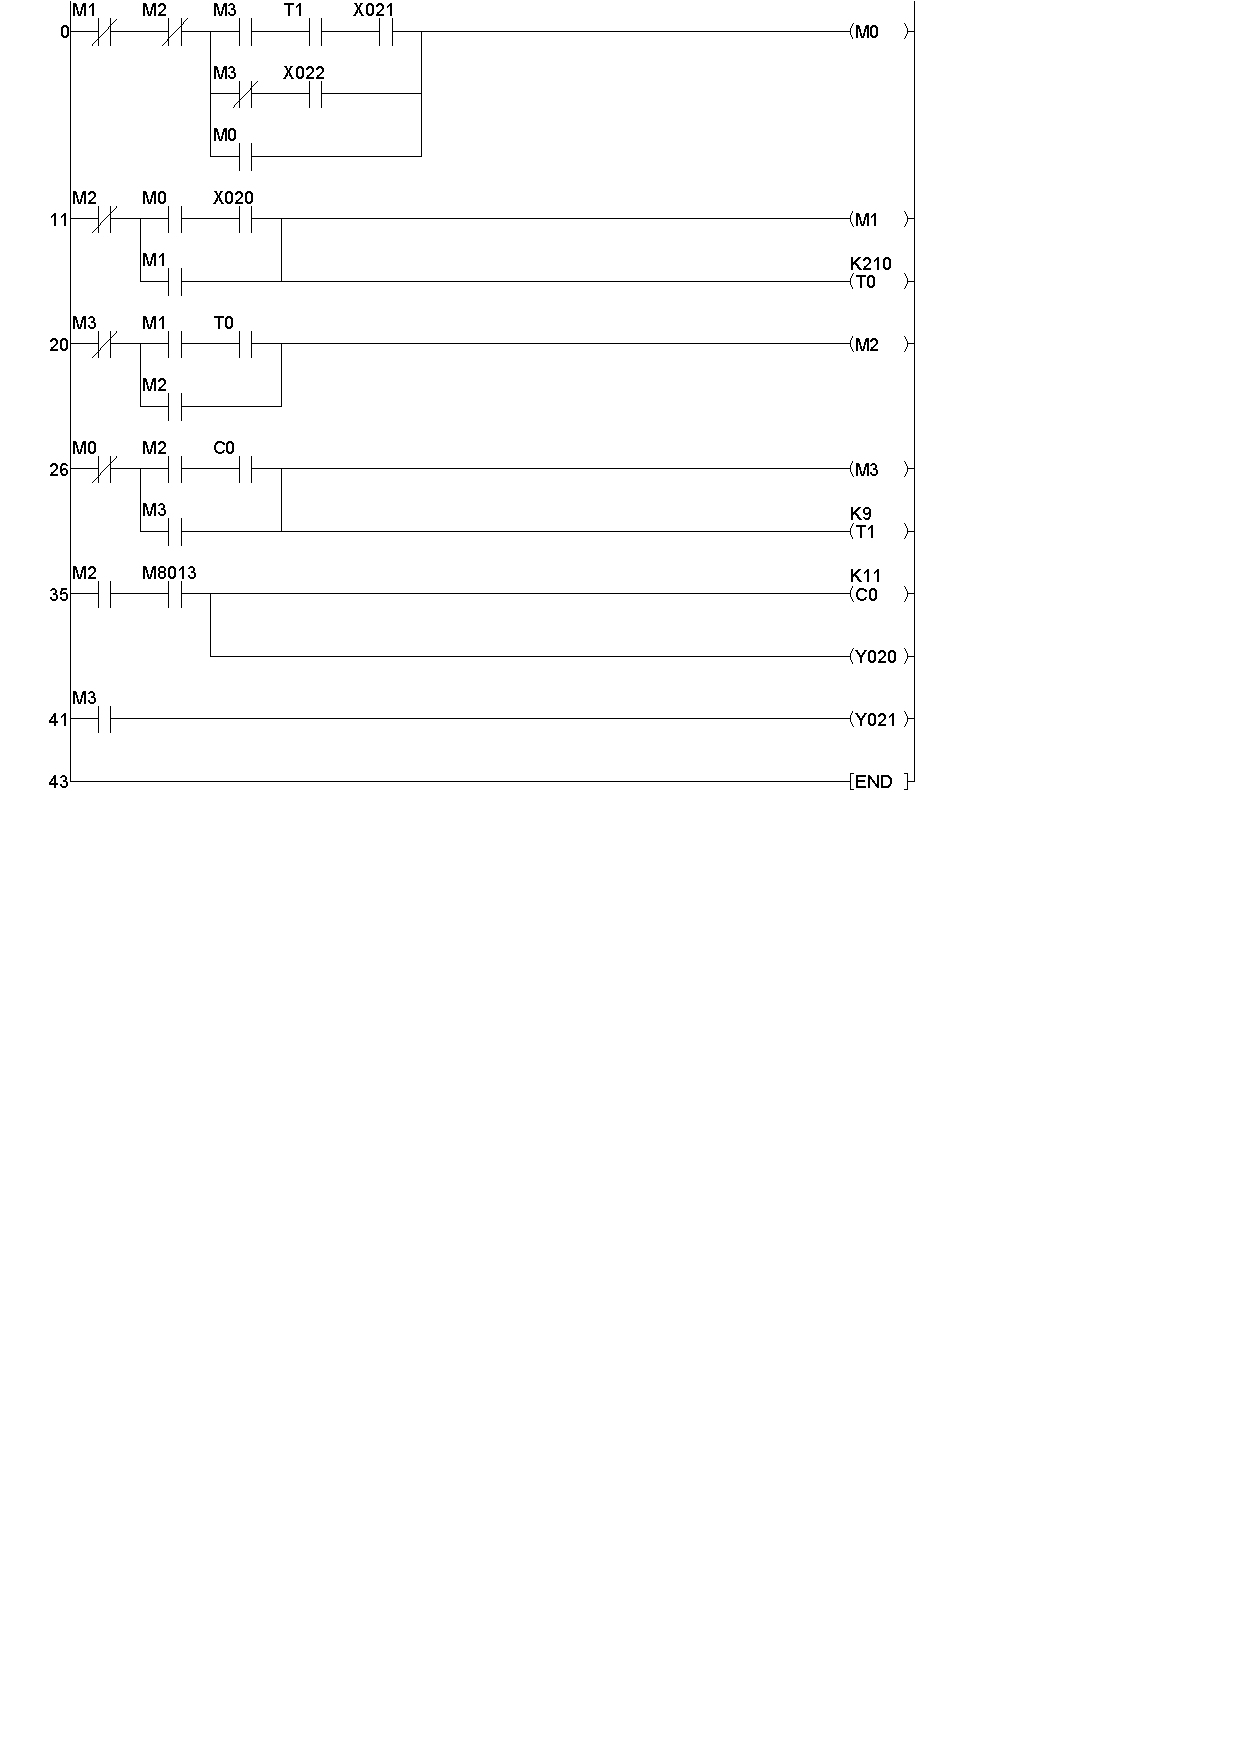
\includegraphics{simulation.pdf}
\end{center}
\end{document}